\section{Results and Discussion}

\subsection{Implementation}
The back end has about 10.5k lines of Python and the app about 5.5k lines of strict TypeScript. The
code is in the project's Git repository (\url{\RepoURL}). Work was divided by module as shown in
Table~\ref{tab:contrib}.
\begin{table}[H]
\centering
\caption{Contribution of group members}
\label{tab:contrib}
\small
\begin{tabularx}{\textwidth}{@{}p{3.6cm}X@{}}
\toprule
\textbf{Member} & \textbf{Main contributions}\\
\midrule
\StudentA{}\newline(\UIDA) & System architecture and database design (schema, migrations, indexes); authentication and role-based access control; natural-language query engine (intent registry Q01--Q30, templates QT01--QT22, clarifications); concurrency control; security audit and fixes; cloud deployment on Render.\\
\StudentB{}\newline(\UIDB) & Timetable extraction pipeline (PDF tables, OCR, Excel/Word adapters); tuning on the college's real PDF (lab groups, legends, noon row, combined B.E.\ page); background worker; conflict detection; extraction and regression tests; performance and load measurements.\\
\StudentC{}\newline(\UIDC) & Cross-platform app (React Native/Expo): role dashboards, weekly view, Ask screen, upload, review and admin screens; laptop/web support and Expo SDK upgrade; mobile and end-to-end tests; documentation, report and poster.\\
\midrule
\textbf{All members} & Requirements analysis and SRS, design reviews with the guide, testing on phones and laptops, demo preparation.\\
\bottomrule
\end{tabularx}
\end{table}


\subsection{Screenshots}
Figures~\ref{fig:realpdf}--\ref{fig:laptop} show the real input and the running app on a phone and a
laptop.
\begin{figure}[H]
\centering
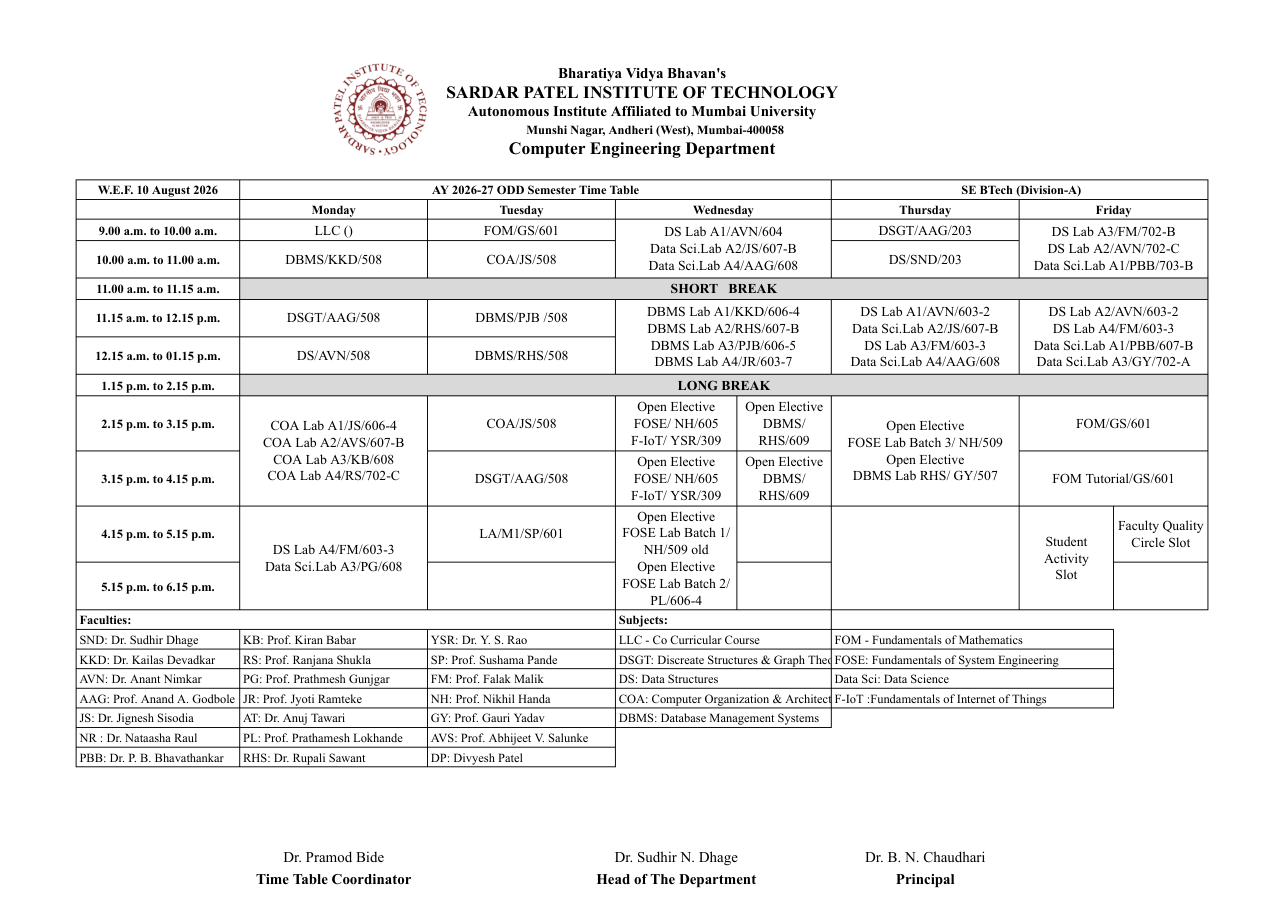
\includegraphics[width=0.75\textwidth]{figures/real-pdf-page1.png}
\caption{Input: page 1 of the college's real timetable PDF (S.E.\ Division A), with stacked lab cells and legend}
\label{fig:realpdf}
\end{figure}

\begin{figure}[H]
\centering
\begin{subfigure}[t]{0.24\textwidth}\centering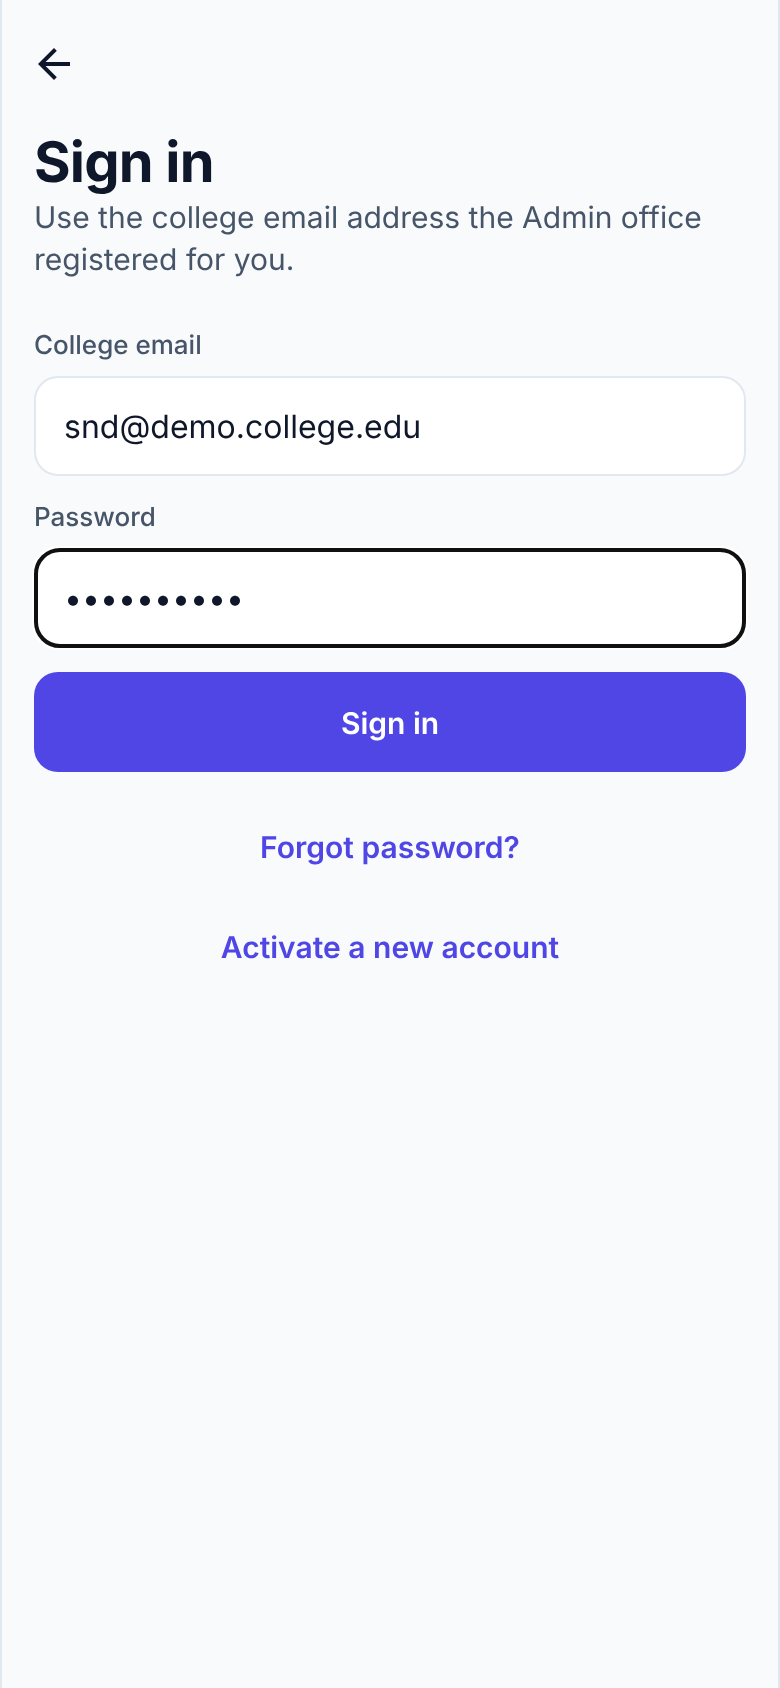
\includegraphics[width=\linewidth]{figures/screens/login.png}\caption{Sign in}\end{subfigure}\hfill
\begin{subfigure}[t]{0.24\textwidth}\centering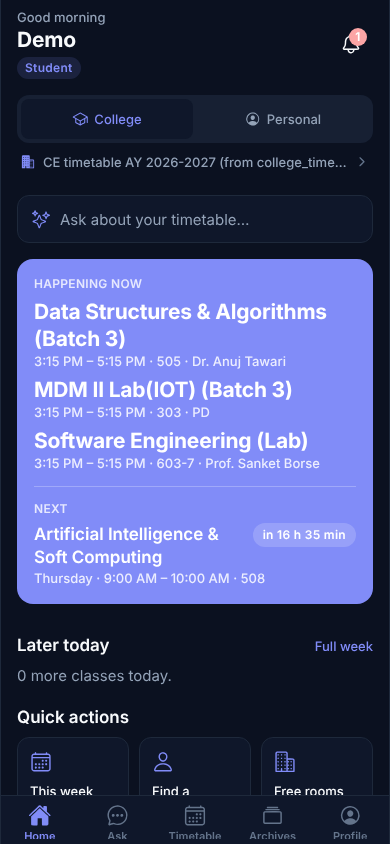
\includegraphics[width=\linewidth]{figures/screens/home-dark.png}\caption{Student home (dark mode): now / next}\end{subfigure}\hfill
\begin{subfigure}[t]{0.24\textwidth}\centering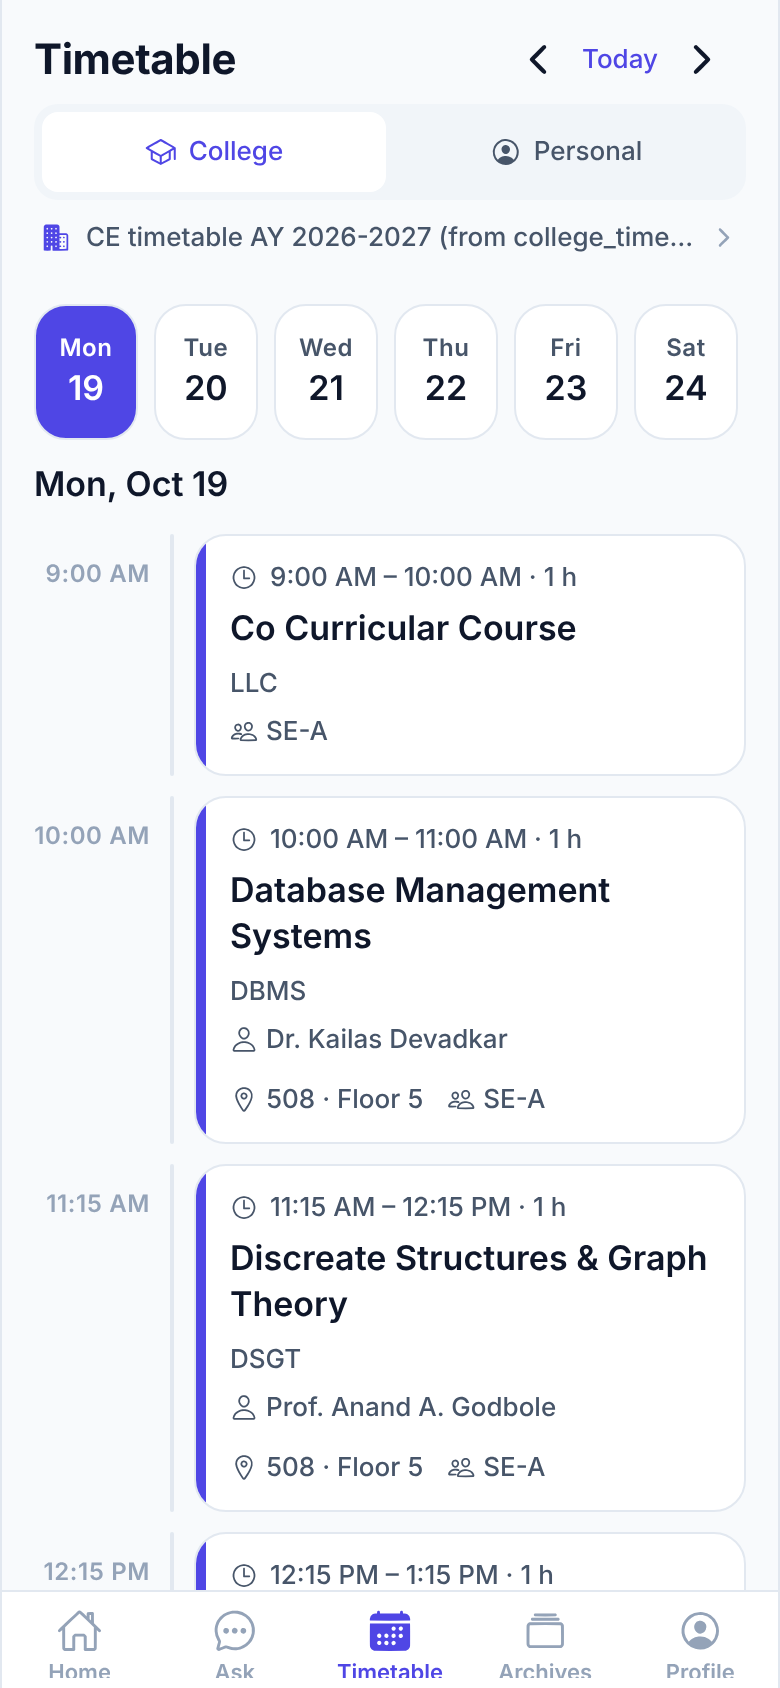
\includegraphics[width=\linewidth]{figures/screens/student-monday.png}\caption{Week view, Monday (SE-A1)}\end{subfigure}\hfill
\begin{subfigure}[t]{0.24\textwidth}\centering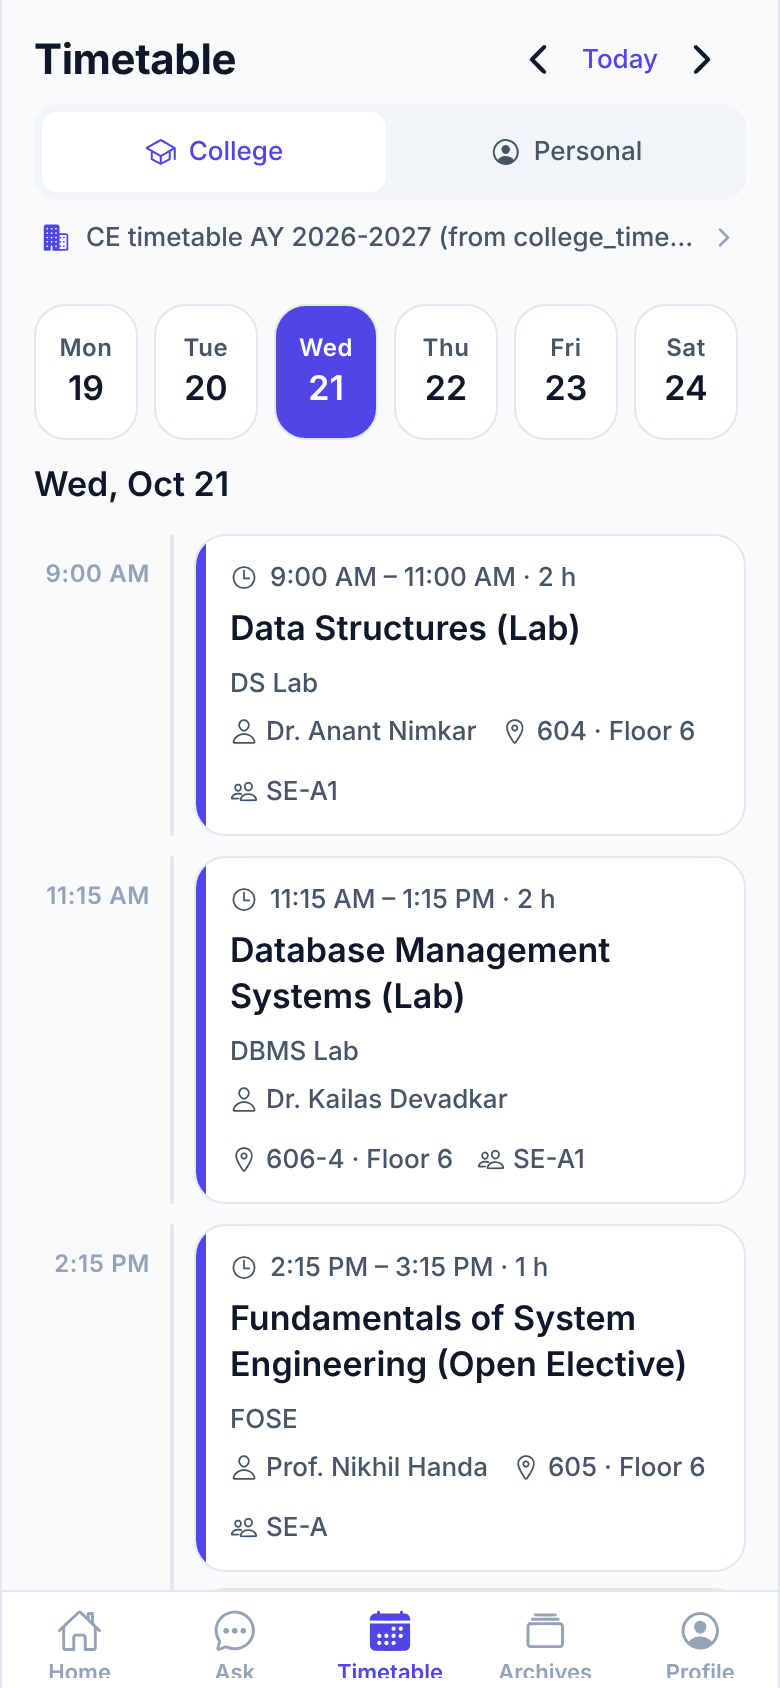
\includegraphics[width=\linewidth]{figures/screens/student-wednesday-lab.png}\caption{Only lab group A1's labs}\end{subfigure}
\caption{Student screens}
\label{fig:screens1}
\end{figure}

\begin{figure}[H]
\centering
\begin{subfigure}[t]{0.24\textwidth}\centering
\includegraphics[width=\linewidth]{figures/screens/class-details.png}\caption{Class details with source page and raw text (LLC: no teacher/room)}\end{subfigure}\hfill
\begin{subfigure}[t]{0.24\textwidth}\centering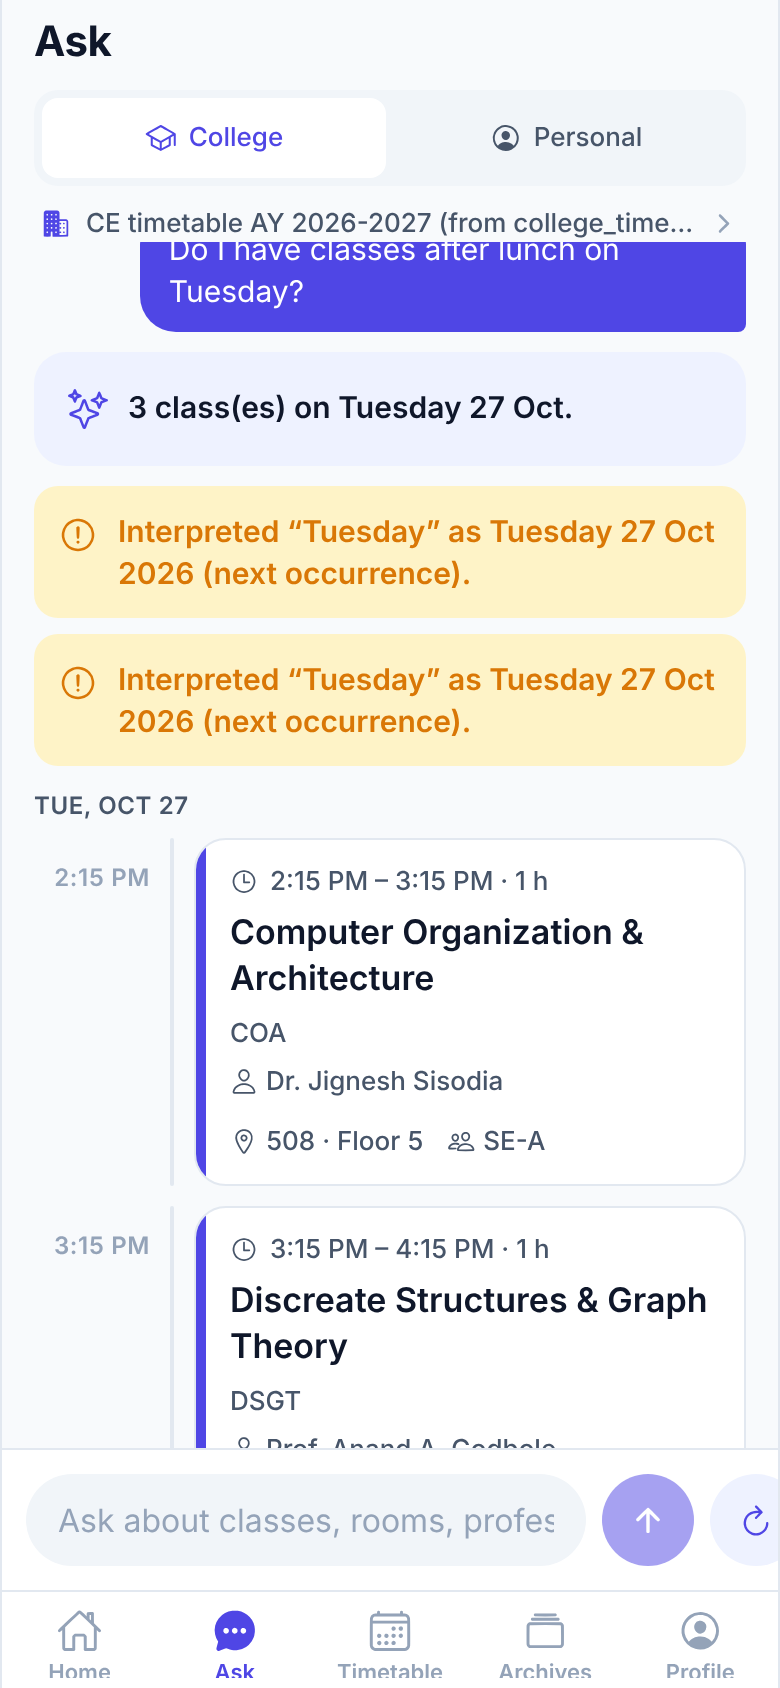
\includegraphics[width=\linewidth]{figures/screens/ask-after-lunch.png}\caption{``Classes after lunch on Tuesday?'' uses SE lunch}\end{subfigure}\hfill
\begin{subfigure}[t]{0.24\textwidth}\centering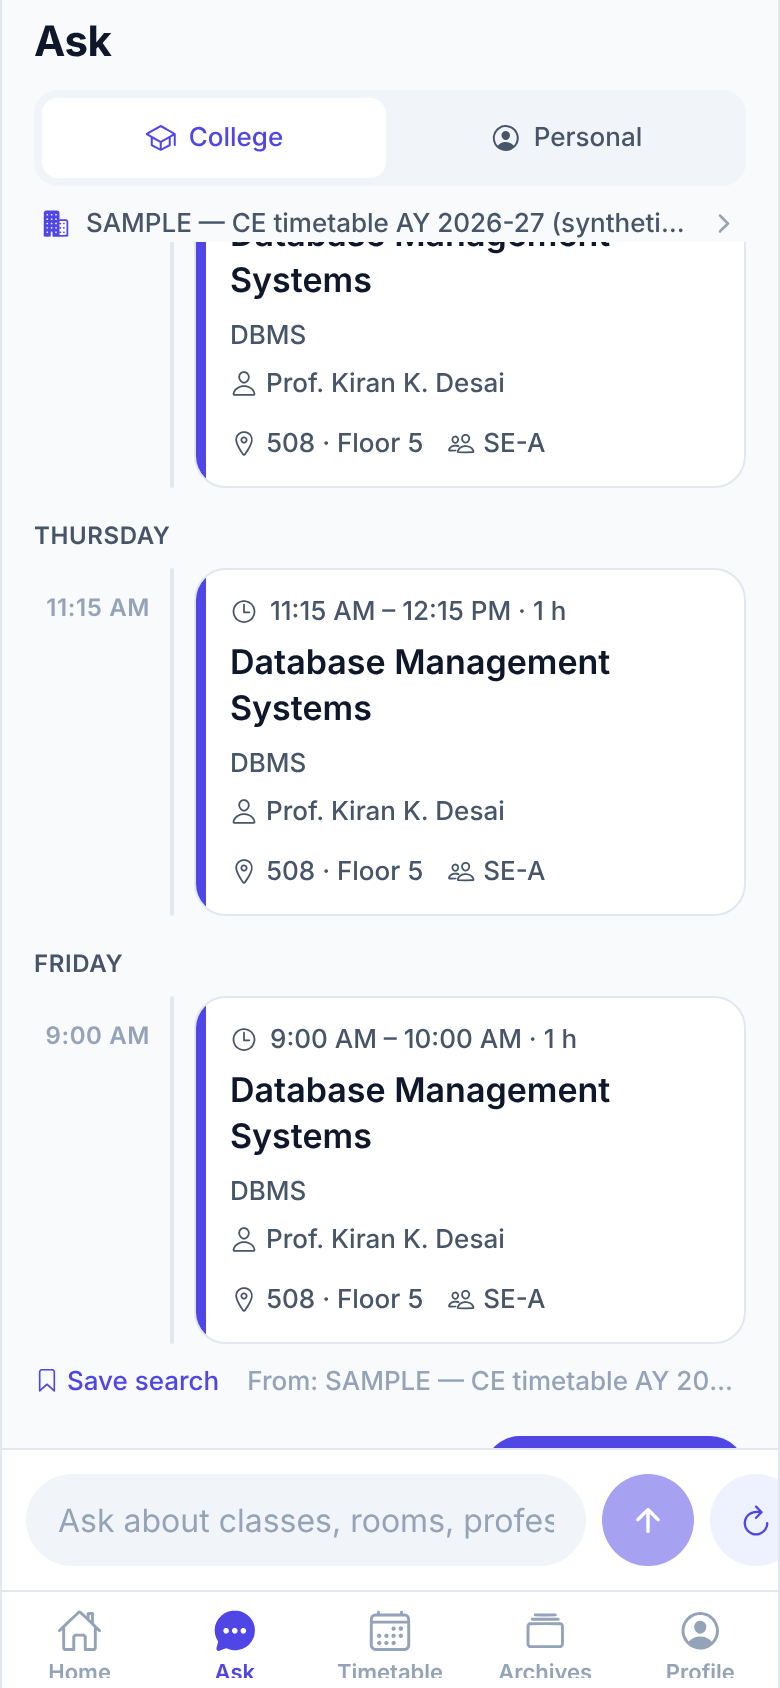
\includegraphics[width=\linewidth]{figures/screens/clarify-ampm.png}\caption{``Am I free at 2?'' asks a.m.\ or p.m.}\end{subfigure}\hfill
\begin{subfigure}[t]{0.24\textwidth}\centering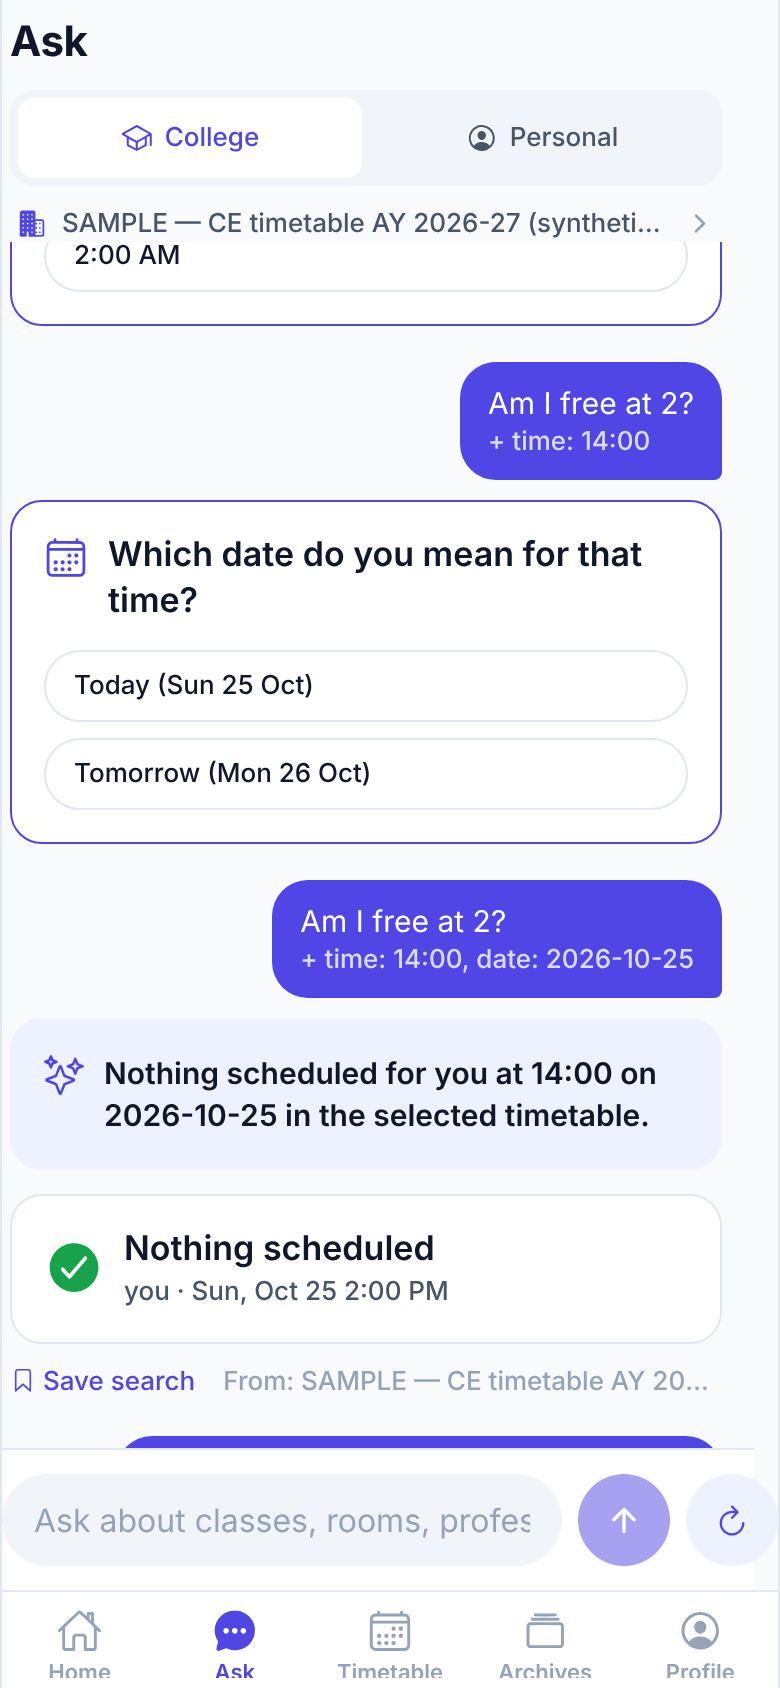
\includegraphics[width=\linewidth]{figures/screens/cross-domain.png}\caption{After choosing 2 PM and the date: answer}\end{subfigure}
\caption{Natural-language search (Ask tab)}
\label{fig:screensask}
\end{figure}

\begin{figure}[H]
\centering
\begin{subfigure}[t]{0.24\textwidth}\centering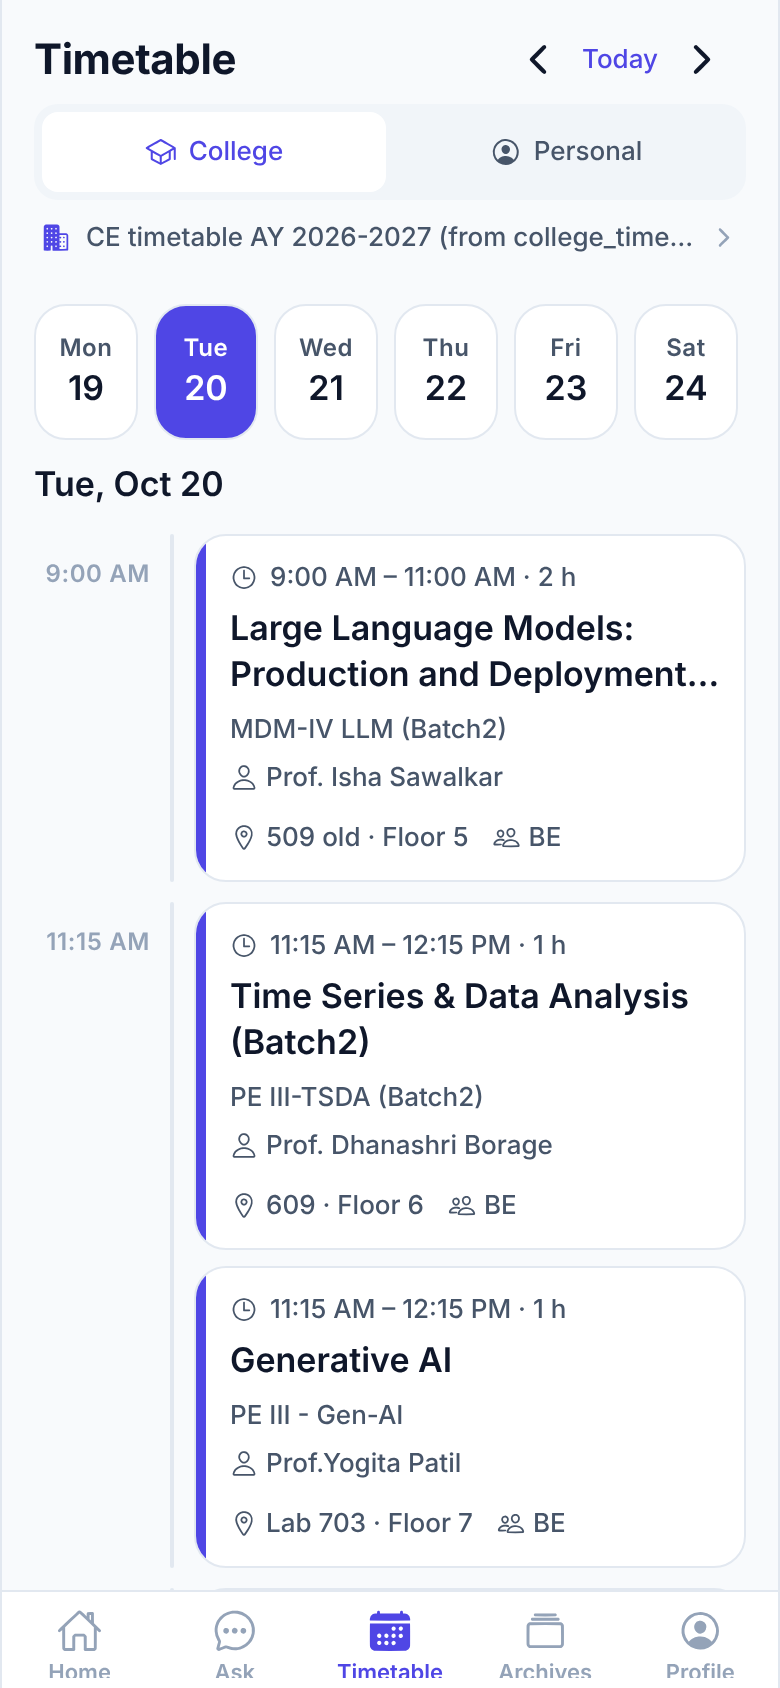
\includegraphics[width=\linewidth]{figures/screens/be-combined.png}\caption{B.E.\ combined electives}\end{subfigure}\hfill
\begin{subfigure}[t]{0.24\textwidth}\centering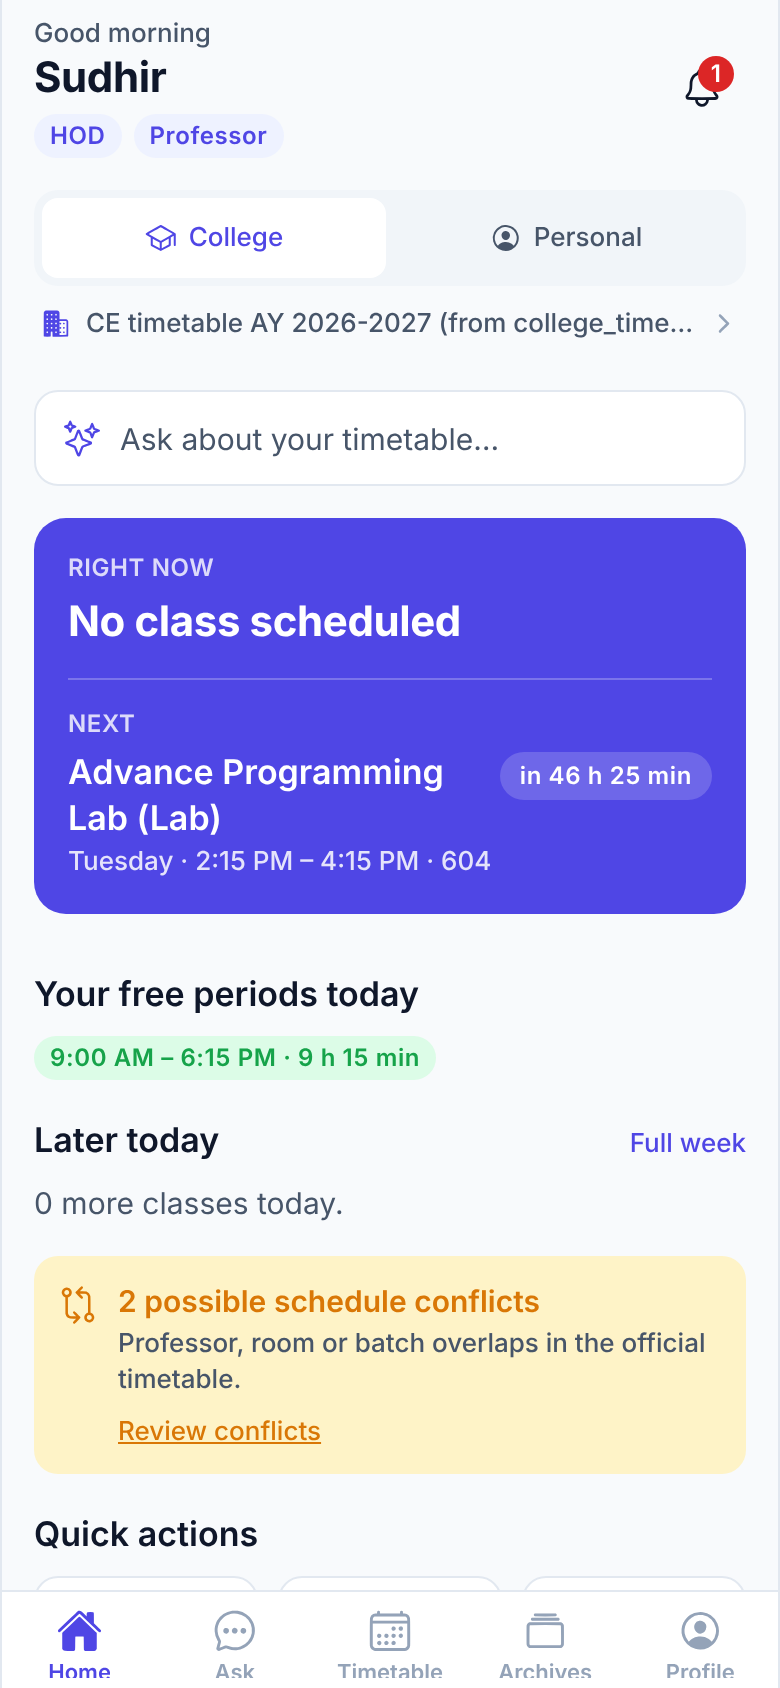
\includegraphics[width=\linewidth]{figures/screens/hod-home.png}\caption{HOD home with conflict alert}\end{subfigure}\hfill
\begin{subfigure}[t]{0.24\textwidth}\centering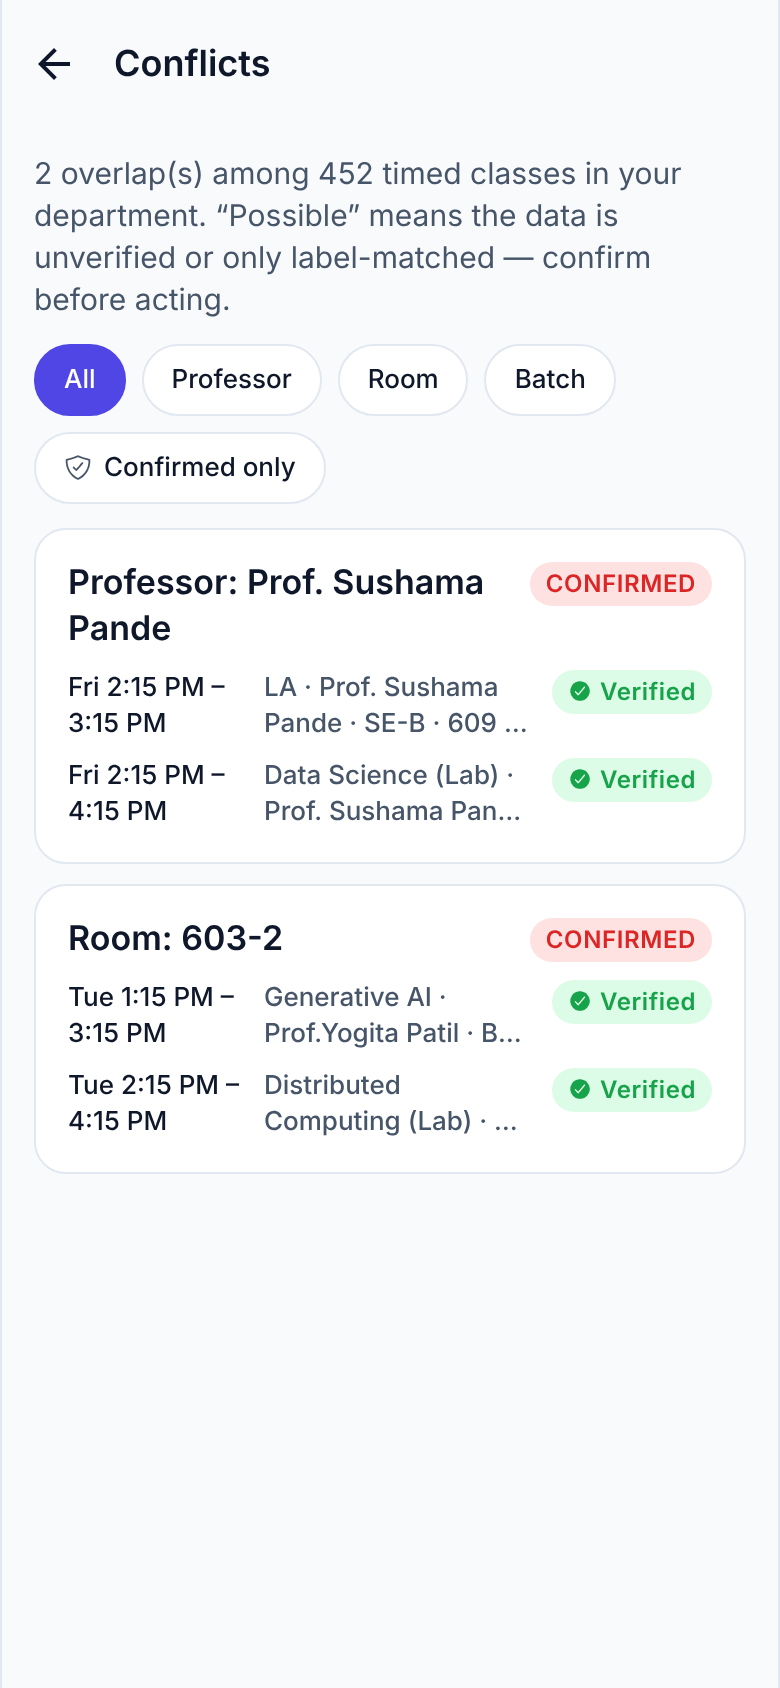
\includegraphics[width=\linewidth]{figures/screens/conflicts.png}\caption{The 2 genuine clashes}\end{subfigure}\hfill
\begin{subfigure}[t]{0.24\textwidth}\centering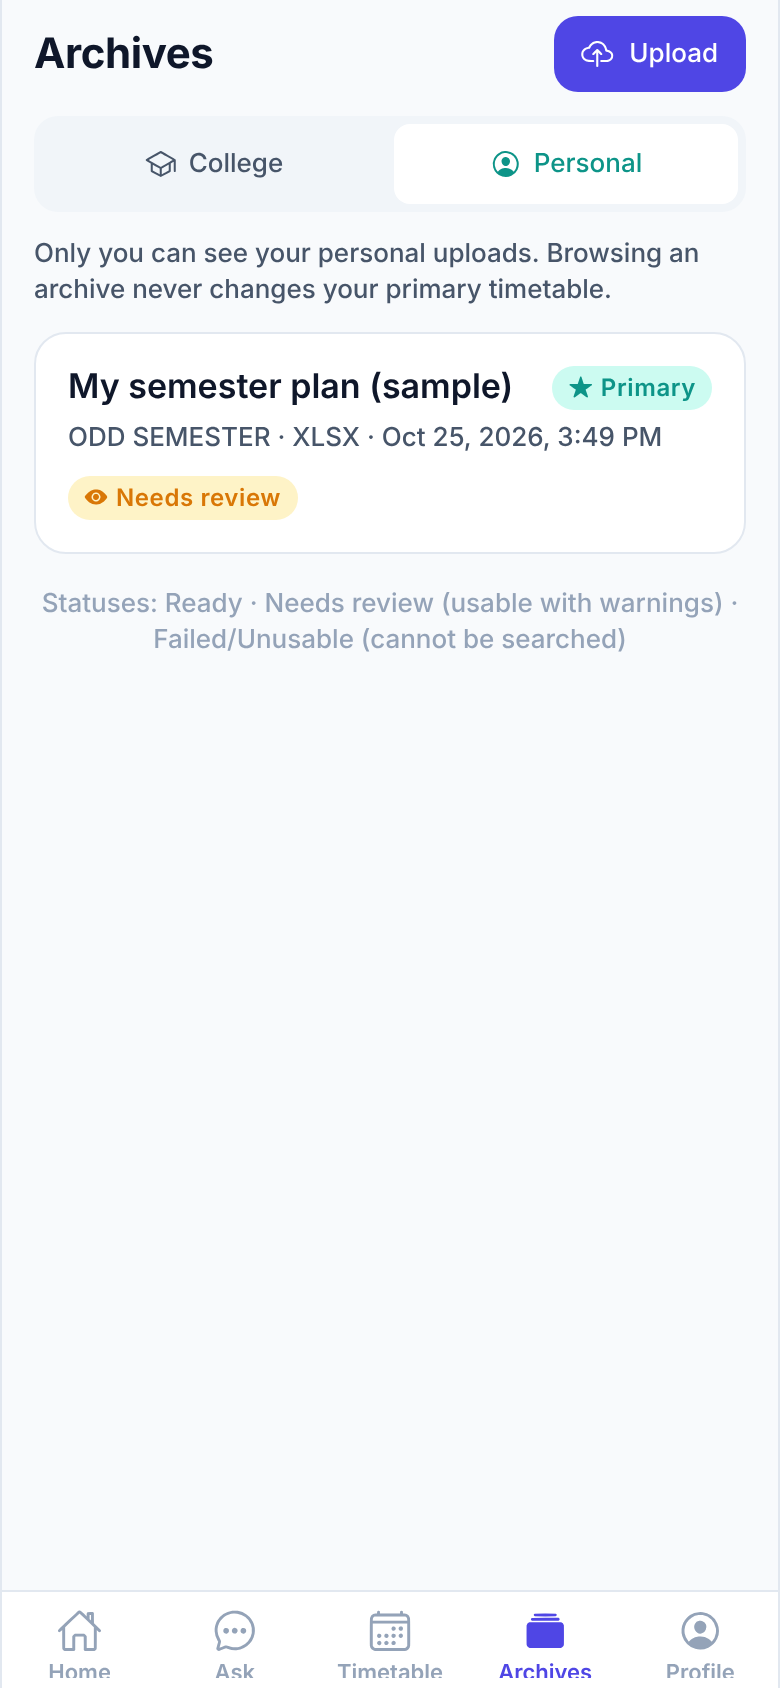
\includegraphics[width=\linewidth]{figures/screens/personal-archives.png}\caption{Personal archives (private)}\end{subfigure}
\caption{Combined classes, HOD view, conflicts and personal domain}
\label{fig:screens2}
\end{figure}

\begin{figure}[H]
\centering
\begin{subfigure}[t]{0.24\textwidth}\centering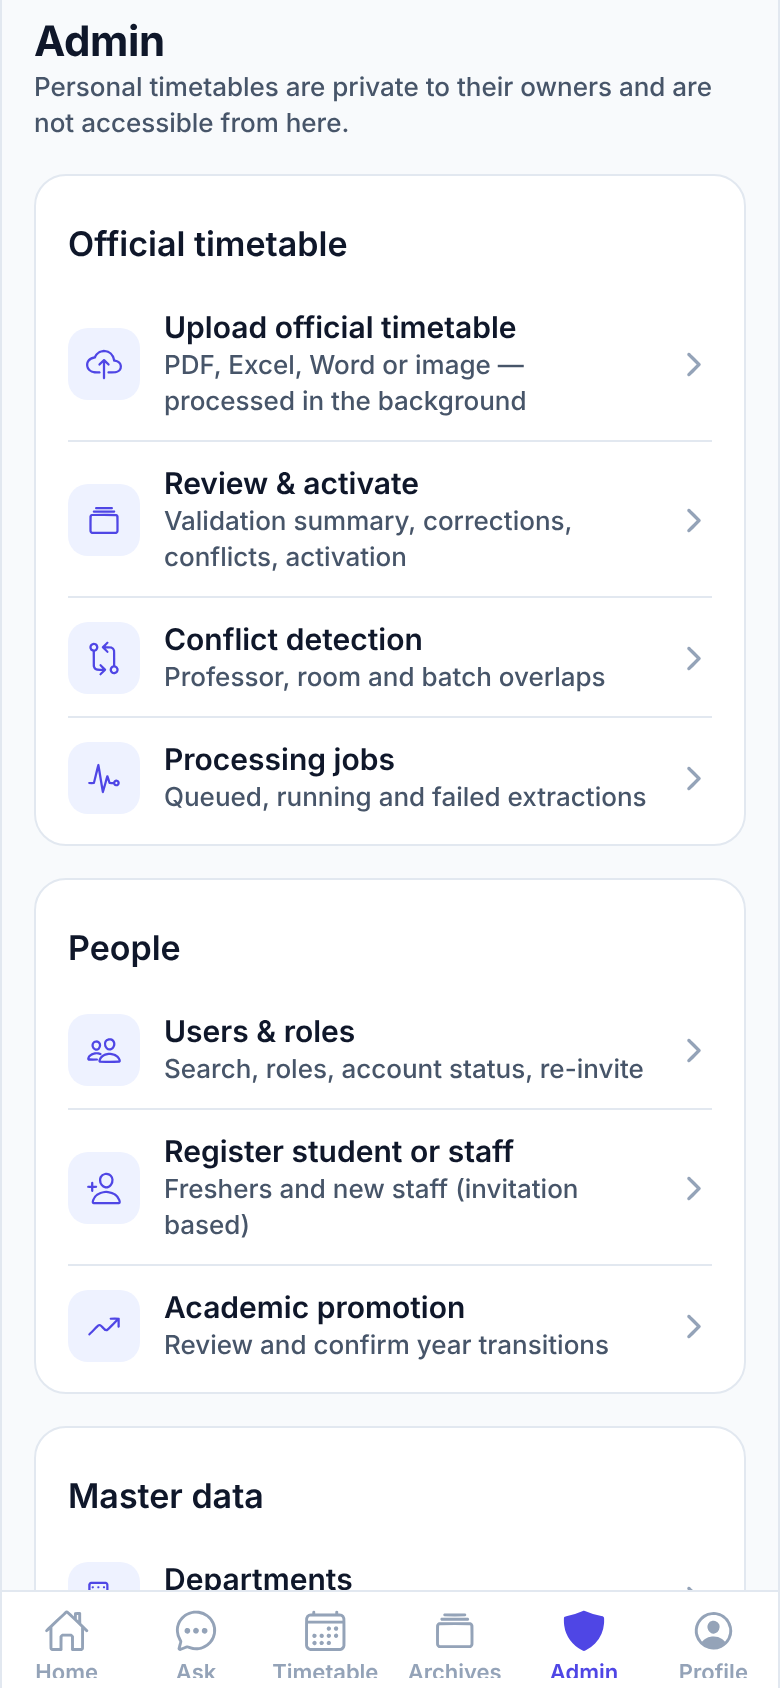
\includegraphics[width=\linewidth]{figures/screens/admin-hub.png}\caption{Admin hub}\end{subfigure}\hfill
\begin{subfigure}[t]{0.24\textwidth}\centering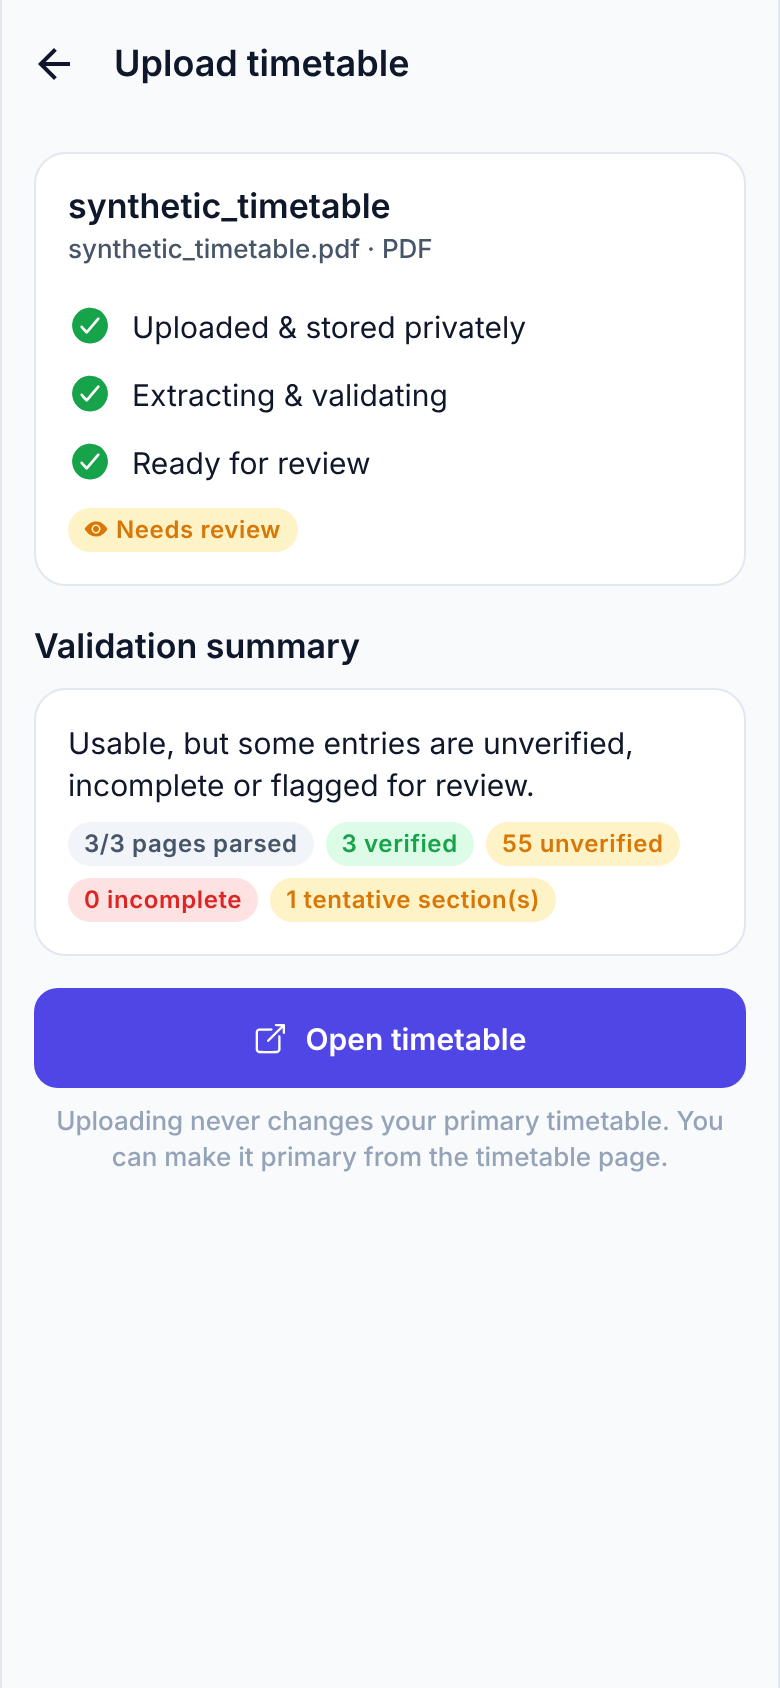
\includegraphics[width=\linewidth]{figures/screens/upload-processed.png}\caption{Upload processed by worker}\end{subfigure}\hfill
\begin{subfigure}[t]{0.24\textwidth}\centering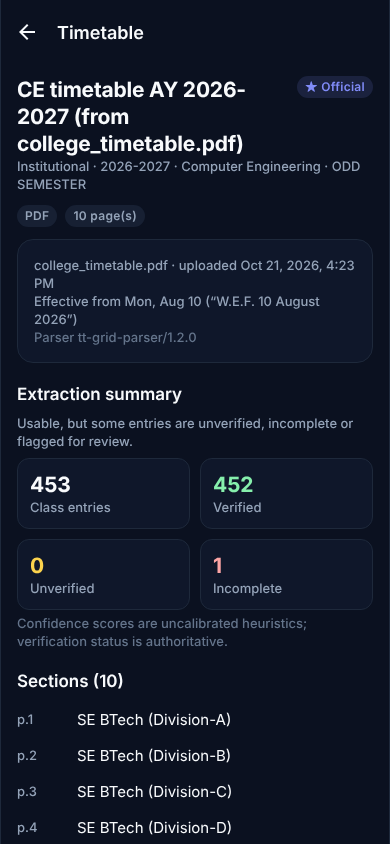
\includegraphics[width=\linewidth]{figures/screens/real-timetable-summary.png}\caption{Real PDF: 453 entries, 452 verified, 10 sections}\end{subfigure}
\caption{Administrator workflow}
\label{fig:screensadmin}
\end{figure}

\begin{figure}[H]
\centering
\begin{subfigure}[t]{0.31\textwidth}\centering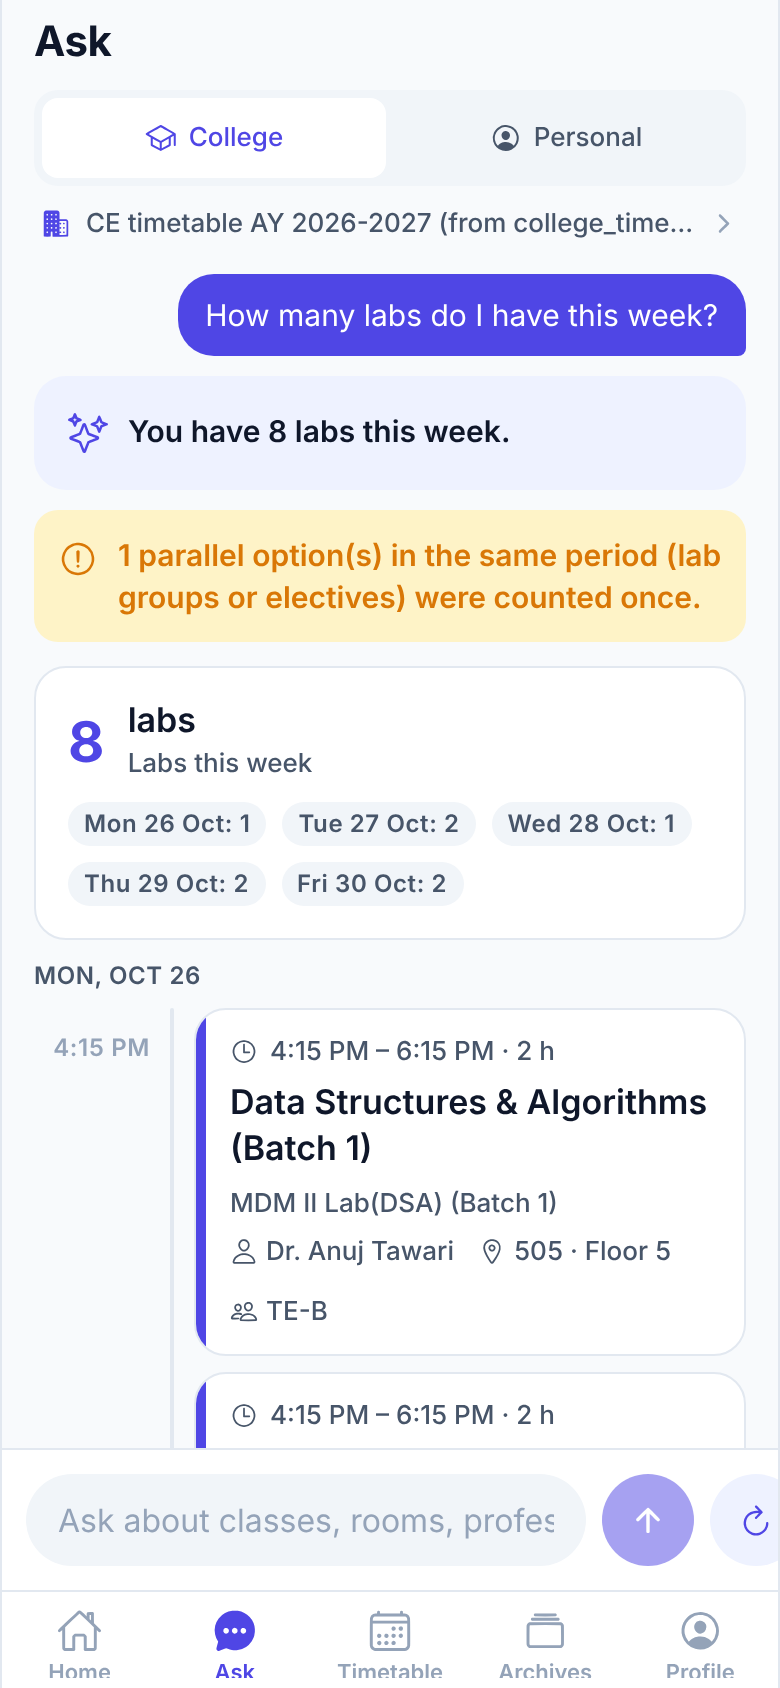
\includegraphics[width=\linewidth]{figures/screens/composed-count.png}\caption{``How many labs do I have this week?'': count with per-day breakdown}\end{subfigure}\hfill
\begin{subfigure}[t]{0.31\textwidth}\centering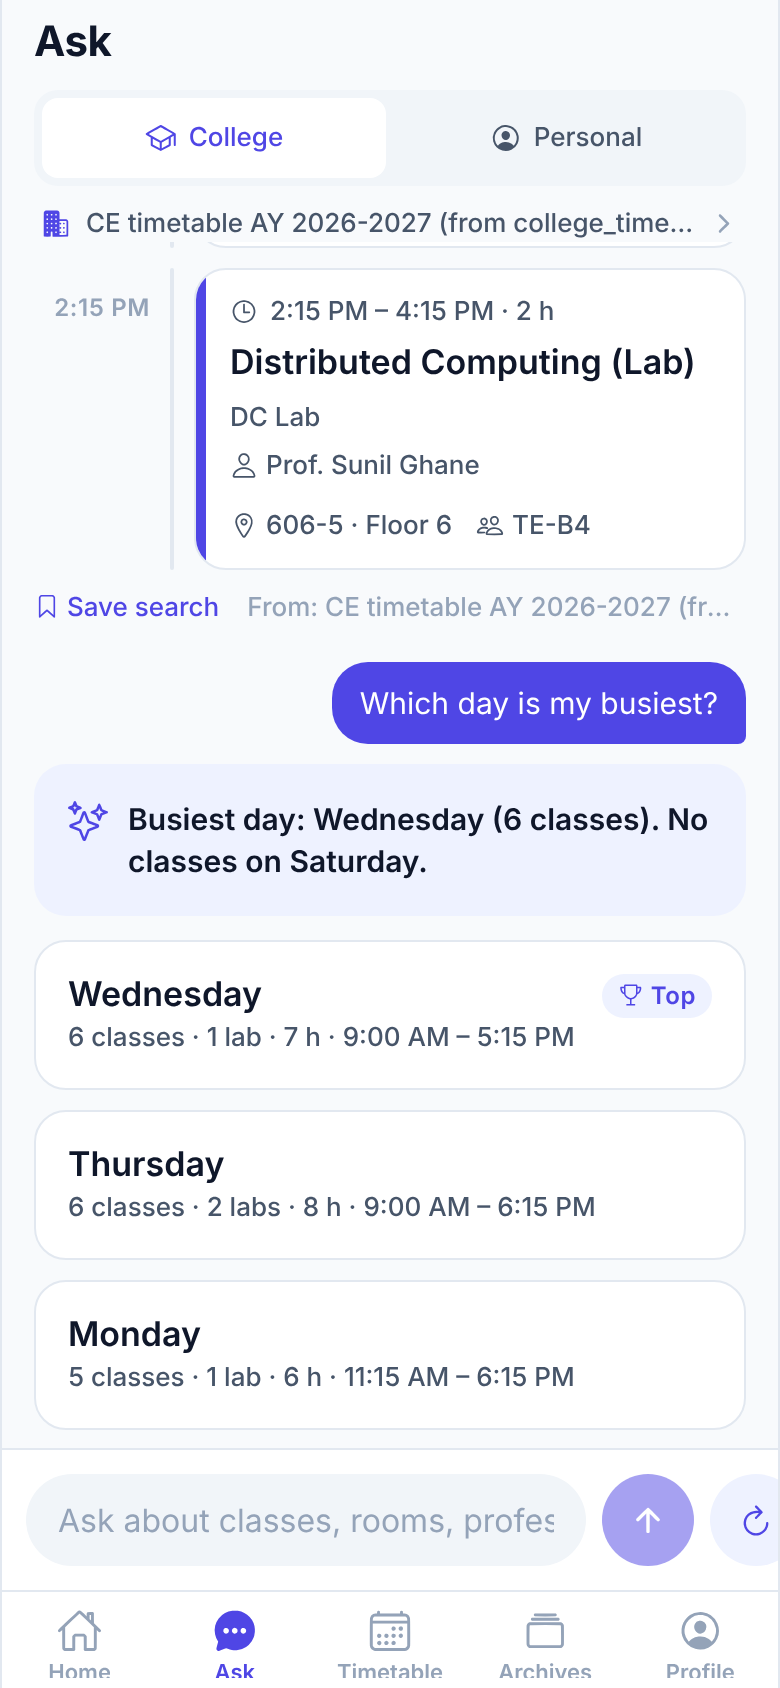
\includegraphics[width=\linewidth]{figures/screens/composed-busiest.png}\caption{``Which day is my busiest?'': day-wise summary}\end{subfigure}\hfill
\begin{subfigure}[t]{0.31\textwidth}\centering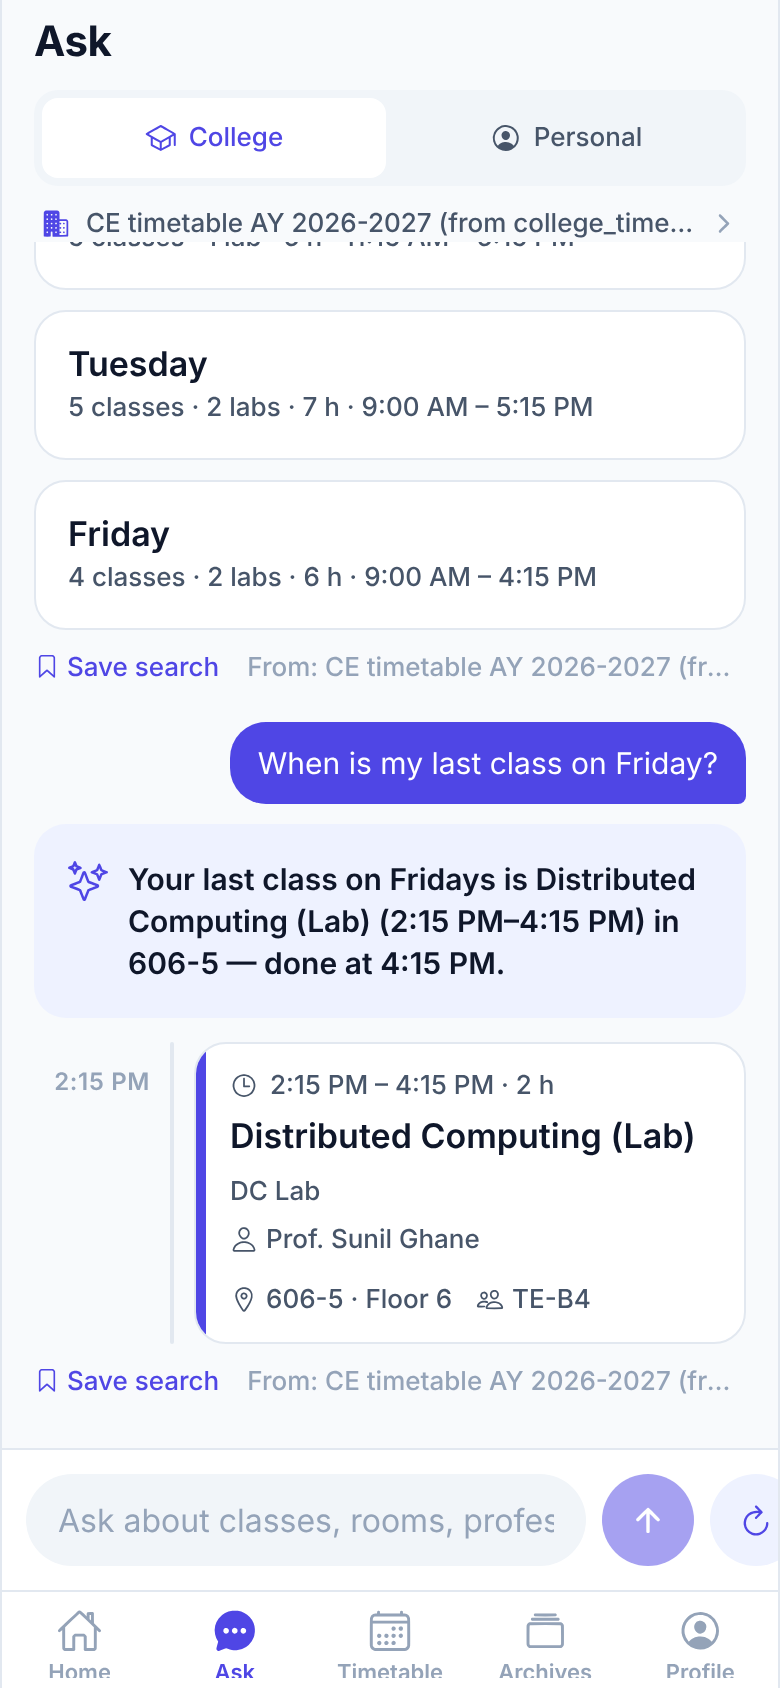
\includegraphics[width=\linewidth]{figures/screens/composed-last.png}\caption{``When is my last class on Friday?''}\end{subfigure}
\caption{Composed query plans answered from the real timetable (TE-B4 student)}
\label{fig:screenscomposed}
\end{figure}

\begin{figure}[H]
\centering
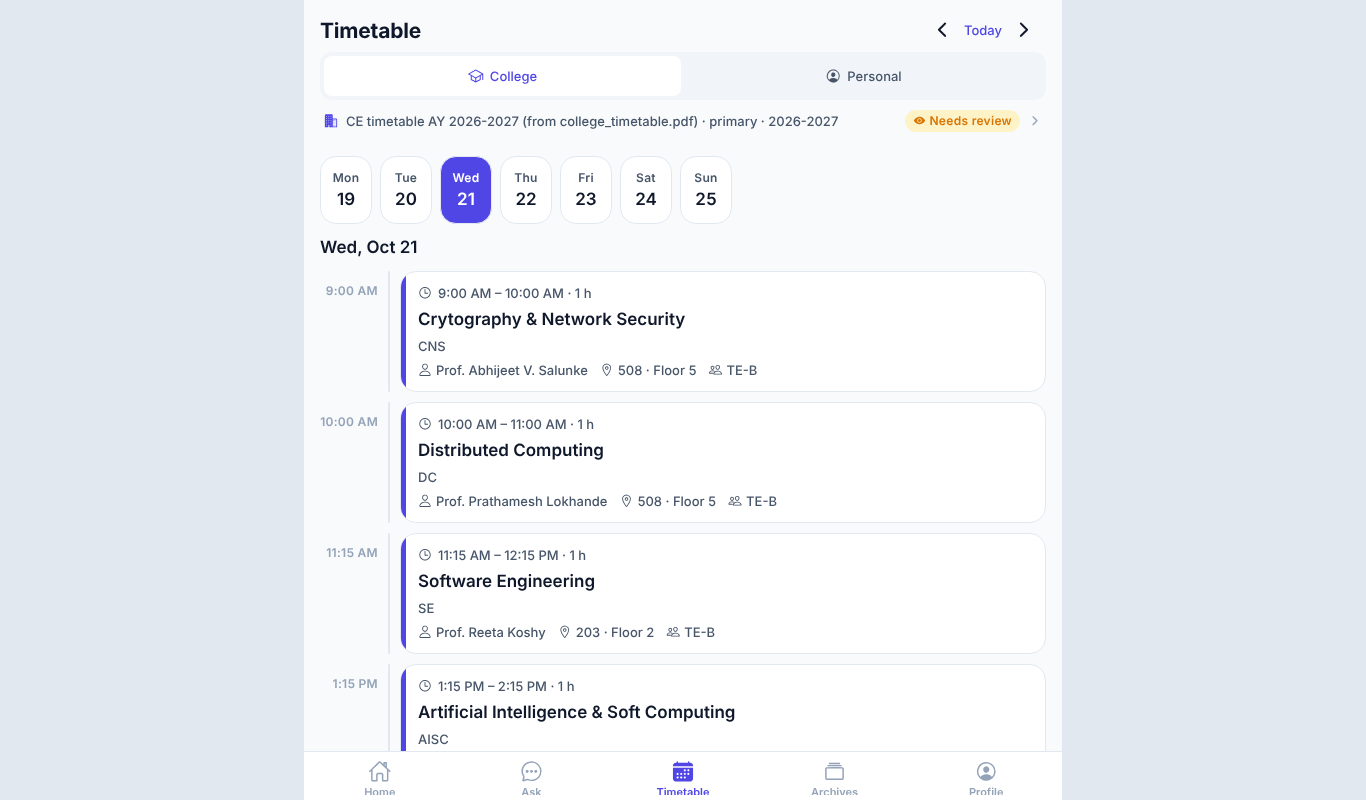
\includegraphics[width=0.8\textwidth]{figures/screens/laptop-timetable.png}
\caption{The same app in a laptop browser}
\label{fig:laptop}
\end{figure}


\subsection{Extraction Results}
The real 10-page PDF produced 570 rows: 453 classes, of which \textbf{452 were verified (99.8\%)} and
one was \textsc{Incomplete} (an M.Tech.\ row with no printed time, flagged instead of guessed), plus
breaks and activities. All 10 pages were parsed and 46 batches, 38 courses, 52 faculty and 42 rooms
were recognised. Table~\ref{tab:extractperf} gives the extraction time.
\begin{table}[H]
\centering
\caption{Extraction performance on the real 10-page PDF (median of 5 runs)}
\label{tab:extractperf}
\small
\begin{tabular}{@{}lr@{}}
\toprule
\textbf{Metric} & \textbf{Value}\\
\midrule
Pages / rows produced & 10 / 570 (453 classes)\\
Extraction time, whole pipeline & 1.65 s (runs: 1.72, 1.65, 1.64, 1.69, 1.64 s)\\
Per page & $\approx$0.17 s\\
Peak memory & 82 MB\\
\bottomrule
\end{tabular}
\end{table}


\subsection{Clash Detection Results}
A naive pairwise check reported 542 overlaps, almost all intended (parallel lab batches, electives,
combined sessions). The intended-overlap rules reduced this to 25 and then to exactly \textbf{2
genuine clashes} (Figure~\ref{fig:conflictbar}), both confirmed by hand in the PDF:
(1) \emph{Friday 2:15--3:15}, Prof.\ Sushama Pande is assigned to SE-B in 609 and SE-C's Data Science
lab in 606-4; (2) \emph{Tuesday 2:15--3:15}, room 603-2 is used by a B.E.\ elective and a T.E.\ lab.
\begin{figure}[H]
\centering
\begin{tikzpicture}
\begin{axis}[ybar,width=0.9\textwidth,height=5.2cm,bar width=16pt,ymin=0,ymax=680,
  symbolic x coords={Naive overlaps,After rule set 1,After rule set 2},xtick=data,
  nodes near coords,ylabel={Reported conflicts},enlarge x limits=0.25,title={\small Conflict reports on the real PDF}]
\addplot[fill=spitblue!60] coordinates {(Naive overlaps,542) (After rule set 1,25) (After rule set 2,2)};
\end{axis}
\end{tikzpicture}
\caption{Effect of intended-overlap rules: from 542 raw overlaps to the 2 genuine clashes}
\label{fig:conflictbar}
\end{figure}


\subsection{Query Results and Performance}
Questions are answered in 37--47~ms (median) for a single user (Table~\ref{tab:latency}). Under load,
throughput peaks at about 60 requests per second with 8 parallel clients, and even at 32 clients every
answer was correct (Table~\ref{tab:loadresults}, Figure~\ref{fig:load}). The API worker uses about
115~MB of memory and the whole database is 12~MB.
\begin{table}[H]
\centering
\caption{Single-user search latency per question type (50 requests each)}
\label{tab:latency}
\small
\setlength{\tabcolsep}{4pt}\begin{tabular}{@{}llrrr@{}}
\toprule
\textbf{Intent} & \textbf{Question} & \textbf{Results} & \textbf{p50 (ms)} & \textbf{p95 (ms)}\\
\midrule
Q10 Next class & What is my next class? & 1 & 42 & 52\\
Q02 Day timetable & What are my classes on Monday? & 5 & 44 & 52\\
Q06 Course search & Find all DBMS classes & 7 & 45 & 51\\
Q11 After lunch & Do I have classes after lunch on Tuesday? & 3 & 47 & 54\\
Q15 Professor schedule & What is my schedule on Monday? & 3 & 37 & 46\\
Q22 Free rooms & Which rooms are free at 10~am today? & 20 & 43 & 51\\
Q20 Room schedule & Show the schedule of room 508 on Monday & 8 & 41 & 49\\
\bottomrule
\end{tabular}
\end{table}

\begin{table}[H]
\centering
\caption{Load test with increasing concurrent clients (4 API workers)}
\label{tab:loadresults}
\small
\begin{tabular}{@{}rrrrrrr@{}}
\toprule
\textbf{Clients} & \textbf{Requests} & \textbf{Wrong} & \textbf{req/s} & \textbf{p50 (ms)} & \textbf{p95 (ms)} & \textbf{CPU (\%)}\\
\midrule
1 & 30 & 0 & 18.6 & 49 & 57 & 31\\
2 & 60 & 0 & 25.4 & 75 & 90 & 32\\
4 & 120 & 0 & 46.5 & 64 & 90 & 48\\
8 & 240 & 0 & 60.4 & 90 & 141 & 63\\
16 & 480 & 0 & 54.1 & 183 & 354 & 62\\
32 & 960 & 0 & 57.4 & 410 & 635 & 76\\
\bottomrule
\end{tabular}
\end{table}

\begin{figure}[H]
\centering
\begin{tikzpicture}
\begin{axis}[width=0.48\textwidth,height=6cm,xmode=log,log basis x=2,xtick={1,2,4,8,16,32},
  xticklabels={1,2,4,8,16,32},xlabel={Concurrent clients},ylabel={Throughput (req/s)},
  ymin=0,ymax=70,grid=major,title={\small Throughput}]
\addplot[thick,mark=*,color=spitblue] coordinates {(1,18.6)(2,25.4)(4,46.5)(8,60.4)(16,54.1)(32,57.4)};
\end{axis}
\end{tikzpicture}\hfill
\begin{tikzpicture}
\begin{axis}[width=0.48\textwidth,height=6cm,xmode=log,log basis x=2,xtick={1,2,4,8,16,32},
  xticklabels={1,2,4,8,16,32},xlabel={Concurrent clients},ylabel={Latency (ms)},
  ymin=0,grid=major,legend pos=north west,legend style={font=\scriptsize},title={\small Latency}]
\addplot[thick,mark=*,color=spitblue] coordinates {(1,49)(2,75)(4,64)(8,90)(16,183)(32,410)};
\addplot[thick,mark=square*,color=orange] coordinates {(1,57)(2,90)(4,90)(8,141)(16,354)(32,635)};
\legend{p50,p95}
\end{axis}
\end{tikzpicture}
\caption{Throughput and latency under increasing concurrent load (measured)}
\label{fig:load}
\end{figure}


\subsection{Testing}
179 back-end tests run against a real PostgreSQL database, the app has 20 Jest tests and compiles
under strict TypeScript, and 45 end-to-end checks run against the live API; all pass.
Table~\ref{tab:testcases} lists the main test cases.
\begingroup\footnotesize
\setlength{\tabcolsep}{3pt}
\begin{longtable}{@{}p{1.15cm}p{1.2cm}>{\raggedright\arraybackslash}p{4.4cm}>{\raggedright\arraybackslash}p{3.6cm}>{\raggedright\arraybackslash}p{2.1cm}p{0.6cm}>{\raggedright\arraybackslash}p{2.3cm}@{}}
\caption{Test case specification}\label{tab:testcases}\\
\toprule
\textbf{TC} & \textbf{Req.} & \textbf{Scenario (input)} & \textbf{Expected result} & \textbf{Actual} & \textbf{P/F} & \textbf{Evidence}\\
\midrule
\endfirsthead
\toprule
\textbf{TC} & \textbf{Req.} & \textbf{Scenario (input)} & \textbf{Expected result} & \textbf{Actual} & \textbf{P/F} & \textbf{Evidence}\\
\midrule
\endhead
TC-01 & FR-01 & Wrong password vs unknown user (Two bad logins) & Same generic error & As expected & P & test\_\allowbreak{}auth\\
TC-02 & FR-01 & Refresh-token reuse (Reuse rotated token) & Whole family revoked, 401 & As expected & P & test\_\allowbreak{}auth\\
TC-03 & FR-02 & Role escalation (Student sends \texttt{roles:[ADMIN]}) & Ignored; admin APIs 403 & As expected & P & test\_\allowbreak{}auth\\
TC-04 & FR-03 & Wrong file type (Text file named \texttt{.pdf}) & Rejected, nothing stored & As expected & P & test\_\allowbreak{}extraction\\
TC-05 & FR-03 & Upload does not change primary (Upload new file) & Primary unchanged & As expected & P & test\_\allowbreak{}uploads\\
TC-06 & FR-03 & Retry same upload (Same client\_\allowbreak{}request\_\allowbreak{}id twice) & One archive record & As expected & P & test\_\allowbreak{}uploads\\
TC-07 & FR-04 & Real PDF extraction (10-page college PDF) & $\geq$95\% verified & 452/453 (99.8\%) & P & test\_\allowbreak{}college\_\allowbreak{}seed\\
TC-08 & FR-04 & Stacked lab cell (Cell with A1--A4) & 4 entries, own room/teacher & As expected & P & test\_\allowbreak{}reference\_\allowbreak{}pdf\\
TC-09 & FR-04 & Noon row typo (``12.15 a.m.\ to 01.15 p.m.'') & 12:15--13:15 with visible note & As expected & P & test\_\allowbreak{}reference\_\allowbreak{}pdf\\
TC-10 & FR-04 & Scanned PDF (Image-only PDF) & OCR, entries \textsc{Unverified} & As expected & P & test\_\allowbreak{}extraction\\
TC-11 & FR-05 & No-table PDF (Plain text PDF) & \textsc{Unusable}, cannot be primary & As expected & P & test\_\allowbreak{}extraction\\
TC-12 & FR-06 & Correction audited (Admin edits room) & Original kept, audit row & As expected & P & test\_\allowbreak{}uploads\\
TC-13 & FR-07 & Concurrent activation (2 threads activate) & Exactly one default & As expected & P & test\_\allowbreak{}academics\\
TC-14 & FR-09 & Dashboard = query (Home vs ``next class?'') & Identical entry & As expected & P & test\_\allowbreak{}query\_\allowbreak{}engine\\
TC-15 & FR-10 & Lab group isolation (SE-A1, Wednesday) & Only A1 labs & As expected & P & test\_\allowbreak{}college\_\allowbreak{}seed\\
TC-16 & FR-11 & Lunch per year (SE vs TE ``after lunch'') & 14:15 vs 13:15 from PDF & As expected & P & test\_\allowbreak{}college\_\allowbreak{}seed\\
TC-17 & FR-11 & Ambiguous time (``Am I free at 2?'') & Clarification a.m./p.m. & As expected & P & test\_\allowbreak{}query\_\allowbreak{}engine, e2e\\
TC-18 & FR-11 & Injection text (``'; DROP TABLE \ldots'') & Treated as text; no SQL run & As expected & P & test\_\allowbreak{}query\_\allowbreak{}engine\\
TC-19 & FR-11 & Cross-domain compare (Q30 question) & UNSUPPORTED, no query executed & As expected & P & test\_\allowbreak{}query\_\allowbreak{}engine\\
TC-20 & FR-12 & Free rooms on a floor (``free rooms on floor 5 at 10'') & Rooms without overlapping class & As expected & P & test\_\allowbreak{}query\_\allowbreak{}engine\\
TC-21 & FR-13 & Clashes in real PDF (Real timetable) & Exactly 2 genuine clashes & 2 (SP Fri; 603-2 Tue) & P & test\_\allowbreak{}college\_\allowbreak{}seed\\
TC-22 & FR-14 & IDOR personal (Other user's timetable id) & 404 + audit & As expected & P & test\_\allowbreak{}uploads\\
TC-23 & FR-15 & Promotion (Preview + confirm) & History kept, new batch & As expected & P & test\_\allowbreak{}academics\\
TC-24 & FR-15 & Concurrent promotion (2 threads) & One open placement & As expected & P & test\_\allowbreak{}academics\\
TC-25 & FR-17 & Student without batch (``next class?'') & Setup-required message & As expected & P & test\_\allowbreak{}college\_\allowbreak{}seed\\
TC-26 & NFR-04 & Reset code in prod (Production, no SMTP) & Code never in response/log & As expected & P & test\_\allowbreak{}deploy\\
TC-27 & NFR-03 & Connectivity probe (\texttt{HEAD /}) & 200 (not 405) & As expected & P & test\_\allowbreak{}deploy\\
TC-28 & NFR-01 & Search latency (50 req/intent) & p50 $<$ 300 ms & 37--47 ms & P & Table~\ref{tab:latency}\\
TC-29 & NFR-03 & Load (32 clients, 960 req) & 0 wrong answers & 0 & P & Table~\ref{tab:loadresults}\\
TC-30 & UI & Full student/HOD flow (Browser, real data) & All steps pass & 24/24 & P & college.e2e.mjs\\
TC-31 & FR-11 & Count with filters (``How many labs do I have this week?'') & Count = distinct lab periods; only labs & As expected & P & test\_\allowbreak{}college\_\allowbreak{}seed\\
TC-32 & FR-11 & First/last (``When is my last class on Friday?'') & Same as max end of the Friday listing & As expected & P & test\_\allowbreak{}college\_\allowbreak{}seed\\
TC-33 & FR-11 & Day-wise ordering (``Which day is my busiest / finish earliest?'') & Days sorted by classes / finish time & As expected & P & test\_\allowbreak{}college\_\allowbreak{}seed\\
TC-34 & FR-02 & ``My labs'' vs another batch (``Show my labs'', ``Show SE-B labs'') & Own lab group for ``my''; SE-B shown when asked & As expected & P & test\_\allowbreak{}college\_\allowbreak{}seed\\
TC-35 & FR-11 & Lunch and free periods (``When is lunch break on Monday?'', ``When am I free on Thursday?'') & Own section's lunch (TE 12:15, SE 1:15); gaps between own classes & As expected & P & test\_\allowbreak{}college\_\allowbreak{}seed\\
TC-36 & FR-11 & Who teaches / what comes after / which floor (``Who teaches software engineering?'') & Teacher names; next class after; floor of room & As expected & P & test\_\allowbreak{}college\_\allowbreak{}seed\\
TC-37 & FR-02 & Open viewing (student asks about SE-B, floor 5, clashes) & Shown to everyone; ``my'' still own batch & As expected & P & test\_\allowbreak{}college\_\allowbreak{}seed\\
TC-38 & FR-11 & Short words not read as names (``Which room is my next class in?'') & Next class, not a batch called ``in'' & As expected & P & test\_\allowbreak{}college\_\allowbreak{}seed\\
\bottomrule
\end{longtable}
\endgroup


\subsection{Comparative Analysis}
Compared with the existing approaches in Table~\ref{tab:compare}, the proposed system is the only one
that reads the published timetable and also answers questions with reproducible, injection-safe
results. Table~\ref{tab:objectives} maps each objective to its evidence.
\begin{table}[H]
\centering
\caption{Objectives mapped to evidence}
\label{tab:objectives}
\small
\begin{tabularx}{\textwidth}{@{}p{0.8cm}Xp{1.9cm}@{}}
\toprule
\textbf{Obj.} & \textbf{Evidence} & \textbf{Status}\\
\midrule
O1 & 99.8\% verified on the real PDF; uncertain values flagged (TC-07, TC-09) & Achieved\\
O2 & PDF, scanned PDF/photo (OCR), XLSX/XLS, CSV, DOCX/DOC through one pipeline (TC-04, TC-10) & Achieved\\
O3 & Five roles, server-side policy, role tests (TC-03), dashboards (Fig.~\ref{fig:screens1}, \ref{fig:screens2}) & Achieved\\
O4 & Specialised operations plus composed query plans (counts, first/last, day-wise, lab/lecture), with clarification (TC-16--TC-19, TC-31--TC-34) & Achieved\\
O5 & 2 genuine clashes, 0 false reports (TC-21) & Achieved\\
O6 & Separate tables; IDOR and isolation tests (TC-22); archives & Achieved\\
O7 & p50 37--47 ms; 0 wrong answers at 32 clients (TC-28, TC-29) & Achieved (dev hardware)\\
O8 & Android/iPhone via Expo Go, laptop browser, Render demo & Achieved; store builds pending\\
O9 & 179 + 20 + 45 e2e steps passing & Achieved\\
\bottomrule
\end{tabularx}
\end{table}


\subsection{Improvements Incorporated after Review}
The following improvements were made after the project reviews and are part of the version
demonstrated at the ESE (Table~\ref{tab:improvements}). Each one is covered by automated tests.
\begin{table}[H]
\centering
\caption{Improvements incorporated before the ESE}
\label{tab:improvements}
\small
\begin{tabularx}{\textwidth}{@{}p{3.6cm}XX@{}}
\toprule
\textbf{Area} & \textbf{Before} & \textbf{After (current version)}\\
\midrule
Question coverage & A fixed list of about 30 question types; counts, ``busiest day'' or ``last lab on Friday'' were refused & Compositional query planner: 17 operations combined with filters, dates, 6 time windows and sorting (Section~5, TC-31--TC-36)\\
Teacher names & Only faculty codes such as AVN were understood & Code, first name, surname or ``Nimkar sir'' all resolve to the same person; spelling variants sharing one code are merged\\
Subject names & Exact subject names only & Partial words and one-letter typos (e.g.\ the PDF's own ``Discreate'') are matched\\
Viewing other timetables & Students saw only their own batch & Anyone can view any teacher's, batch's or room's official timetable through a picker; personal timetables stay private (TC-37)\\
Lunch and free time & Not answerable & Each section's own lunch and the free gaps between one's classes (TC-35)\\
Short words in questions & ``in'', ``at'' or ``is'' were sometimes read as a batch or a name & Stop-word lists prevent these misreadings (TC-38)\\
Explainability & Only the answer was shown & Every answer carries the query plan that produced it\\
\bottomrule
\end{tabularx}
\end{table}


\subsection{Scenario-Based Challenges}
Table~\ref{tab:scenarios} lists realistic situations the system can face in a college and how it
handles each one; every row is backed by a test case or a measured result.
\begingroup
\small
\begin{longtable}{@{}>{\raggedright\arraybackslash}p{4.2cm}>{\raggedright\arraybackslash}p{7.3cm}>{\raggedright\arraybackslash}p{2.6cm}@{}}
\caption{Scenario-based challenges and how the system responds}\label{tab:scenarios}\\
\toprule
\textbf{Scenario} & \textbf{System behaviour} & \textbf{Evidence}\\
\midrule
\endfirsthead
\toprule
\textbf{Scenario} & \textbf{System behaviour} & \textbf{Evidence}\\
\midrule
\endhead
The department releases a revised timetable mid-semester & The admin uploads the new PDF; the old version stays in the archive and the current one keeps serving users until the new one is reviewed and activated & TC-05, TC-06\\
A room changes for one class after publishing & The admin corrects the entry; the original value, the new value, the reason and the admin are stored in an audit record & TC-12\\
The PDF prints the noon row as ``12.15 a.m.\ to 01.15 p.m.'' & Backtracking proves 12:15--13:15 from the neighbouring rows and shows a visible note & TC-09, Alg.~\ref{alg:time}\\
A row has no printed time & The entry is marked \textsc{Incomplete} and is not used in answers, instead of being guessed & Sec.~10.3\\
Only a phone photo or scanned copy is available & OCR reads it and its entries are marked \textsc{Unverified} for review & TC-10\\
A wrong file is uploaded (text renamed to .pdf, or a PDF without a table) & Rejected or marked \textsc{Unusable}; it can never become the official timetable & TC-04, TC-11\\
The same teacher is spelled two ways in the PDF & Entries sharing a faculty code are merged into one person & TC-36\\
One teacher is scheduled in two rooms at once & Reported as a clash to the HOD; the 2 genuine clashes in the real PDF were found & TC-21\\
A student types ``Am I free at 2?'' & The system asks whether 2 a.m.\ or 2 p.m.\ is meant instead of guessing & TC-17\\
A user types SQL such as \texttt{'; DROP TABLE} into the question box & Treated as plain text; no SQL is built from user text & TC-18\\
A student tries to open another user's personal timetable & Returns 404 and the attempt is logged & TC-22\\
A student sends \texttt{roles:[ADMIN]} in a request & Ignored; admin endpoints return 403 & TC-03\\
A stolen refresh token is reused & The whole token family is revoked & TC-02\\
Two admins activate different timetables at the same moment & Exactly one becomes the default; no corrupted state & TC-13\\
Year-end promotion of all students & Preview, then confirm; history is kept and each student has one current placement & TC-23, TC-24\\
A new student has not been assigned a batch yet & A clear ``setup required'' message instead of wrong classes & TC-25\\
Many students open the app at 8:55 a.m. & 32 parallel clients: 57 requests/s, 0 wrong answers & TC-29\\
\bottomrule
\end{longtable}
\endgroup


\subsection{Discussion}
\begin{itemize}
\item \textbf{Real data differs from specifications.} Most extraction work went into conventions found
      only in the real PDF: the mislabelled noon row, codes missing from legends, LLC slots and the
      combined B.E.\ page. Testing on the real document from the start was decisive.
\item \textbf{Honest uncertainty builds trust.} Marking the one entry without a time as
      \textsc{Incomplete}, instead of guessing, kept every automatic answer correct.
\item \textbf{The source document itself had errors.} The two clashes are real errors in the
      published timetable, so the system already adds value for the timetable committee.
\item \textbf{Rules work here if they compose.} A fixed list of question types was limiting; composing
      rules into a query plan removed most of that limit while keeping exact answers in about 40~ms,
      at no API cost and with no injection risk.
\end{itemize}
\newpage
